
% This LaTeX was auto-generated from MATLAB code.
% To make changes, update the MATLAB code and republish this document.

\documentclass[11pt]{article}
\usepackage[utf8]{inputenc}
\usepackage[T1]{fontenc}
\usepackage{amsthm}
\usepackage{enumitem}
\usepackage{amssymb}
\usepackage{amsmath}
\usepackage{amsfonts}
\usepackage[version=4]{mhchem}
\usepackage{stmaryrd}
\usepackage{mathrsfs}
\usepackage{bm}
\usepackage{graphicx}
\usepackage[export]{adjustbox}
\graphicspath{ {./images/} }
\usepackage{algorithm}
\usepackage{algorithmic}
\usepackage{makecell}  % 表格换行
\usepackage{tikz}
\renewcommand{\arraystretch}{1.3} % 将行高增大为原来的 1.3 倍
\usepackage{subcaption}
\captionsetup[subfigure]{labelformat=simple, labelsep=space}
\renewcommand{\thesubfigure}{\alph{subfigure}.} % 生成 a, b 而不是 (a), (b)


\usepackage{hyperref}
\hypersetup{
    colorlinks=true,     % 启用颜色链接
    linkcolor=blue,     % 内部链接的颜色
    citecolor=blue,      % 引用文献的颜色
    urlcolor=blue,       % URL链接的颜色
    linktoc=red,      % 不影响目录链接颜色
}

\usepackage[a4paper, top=1in, bottom=1in, left=1in, right=1in]{geometry}

\title{
{\bf \huge Notes on M\"untz-Jackson Theorem}
%{\bf \large For M\"untz systems on [0,1]}
}
\author{Huaijin Wang}
\date{December 10, 2024}


\begin{document}


\newtheorem{definition}{Definition}[section]
\newtheorem{property}{Property}[section]
\newtheorem{lemma}{Lemma}[section]
\newtheorem{theorem}{Theorem}[section]
\newtheorem{corollary}{Corollary}[section]
\newtheorem{remark}{Remark}[section]
\newtheorem{example}{Example}[]
\newtheorem{notation}{Notation Declaration}[]
\newtheorem{question}{Question}[]
\newtheorem{exercise}{Exercise}[section]
\newtheorem{exercise*}{Exercise}[]

%\maketitle




\newpage



\begin{exercise*}
Let $\Omega = (-1,1)^2$. For $\alpha \in \mathbb{R}$, construct for the problem
\[
\left\{
\begin{aligned}
& \alpha u-\Delta u=1, \quad \forall x \in \Omega, \\
& \left.u\right|_{\Gamma_D}=0, \\
& \left.\frac{\partial u}{\partial n}\right|_{\Gamma_N}=2,
\end{aligned}\right.
\]
respectively a $Q1-$FEM based on the rectangular mesh in Fig.~\subref{mesh-Q1} and a $P1-$FEM based on the triangular mesh in Fig.~\subref{mesh-P1}




\begin{figure}[H]

\begin{subfigure}{0.45\textwidth}
\centering
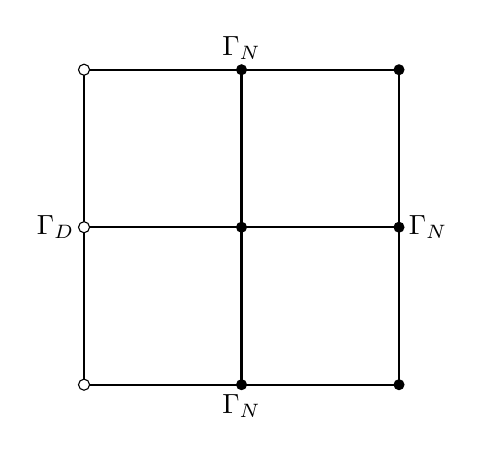
\begin{tikzpicture}[scale=2]

% 绘制矩形边界
\draw[thick] (-1,-1) rectangle (1,1);

% 网格步长
\def\step{1}

% 绘制网格线
\foreach \x in {-1,0,1} {
  \draw[thick] (\x,-1) -- (\x,1);
}
\foreach \y in {-1,0,1} {
  \draw[thick] (-1,\y) -- (1,\y);
}

% 节点位置列表(共9个)
\foreach \x in {-1,0,1} {
  \foreach \y in {-1,0,1} {
    % 判断是否画实心或空心点
    \pgfmathtruncatemacro{\isSolid}{ifthenelse(\x==-1,0,1)}
    % if x==-1, isSolid=0, else, isSolid=1
    \ifnum\isSolid=1
      \fill (\x,\y) circle (1pt); % 实心点
    \else
      \draw[fill=white] (\x,\y) circle (1pt); % 空心点
    \fi
  }
}

\node[left] at (-1,0) {$\Gamma_D$};

\node[below] at (0,-1) {$\Gamma_N$};

\node[above] at (0,1) {$\Gamma_N$};

\node[right] at (1,0) {$\Gamma_N$};

\end{tikzpicture}

\caption{Mesh for $Q1-$FEM.}
\label{mesh-Q1}
\end{subfigure}
\hfill
\begin{subfigure}{0.45\textwidth}
\centering
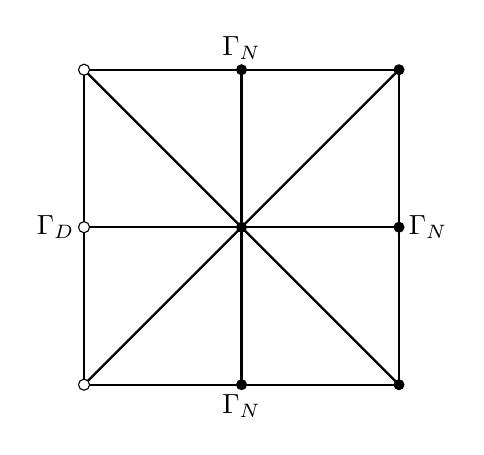
\begin{tikzpicture}[scale=2]

% 绘制矩形边界
\draw[thick] (-1,-1) rectangle (1,1);

% 网格步长
\def\step{1}

% 绘制网格线
\foreach \x in {-1,0,1} {
  \draw[thick] (\x,-1) -- (\x,1);
}
\foreach \y in {-1,0,1} {
  \draw[thick] (-1,\y) -- (1,\y);
}
\draw[thick] (-1,-1) -- (1,1);
\draw[thick] (-1,1) -- (1,-1);


% 节点位置列表(共9个)
\foreach \x in {-1,0,1} {
  \foreach \y in {-1,0,1} {
    % 判断是否画实心或空心点
    \pgfmathtruncatemacro{\isSolid}{ifthenelse(\x==-1,0,1)}
    % if x==-1, isSolid=0, else, isSolid=1
    \ifnum\isSolid=1
      \fill (\x,\y) circle (1pt); % 实心点
    \else
      \draw[fill=white] (\x,\y) circle (1pt); % 空心点
    \fi
  }
}

\node[left] at (-1,0) {$\Gamma_D$};

\node[below] at (0,-1) {$\Gamma_N$};

\node[above] at (0,1) {$\Gamma_N$};

\node[right] at (1,0) {$\Gamma_N$};

\end{tikzpicture}

\caption{Mesh for $P1-$FEM.}
\label{mesh-P1}
\end{subfigure}

\end{figure}

\end{exercise*}



\begin{proof}[Solution]
Let $V=\left\{v\left|v \in H^1(\Omega), v\right|_{\Gamma_D}=0\right\}$. The variational form reads
\[
\left\{
\begin{aligned}
& \text{Find}\ u\in V\ \text{s.t.} \\
& a(u,v) = \mathcal{F}(v),\ \forall v\in V,
\end{aligned}
\right .
\]
where $a(u, v)=\alpha(u, v)+(\nabla u, \nabla v)$ and $\mathcal{F}(v) = (1,v)+(2,v)_{\Gamma_N}$. Let $V_h\subset V$ be the finite dimensional space. Then the Galerkin approximation reads
\begin{equation}
\left\{
\begin{aligned}
& \text{Find}\ u_h\in V_h\ \text{s.t.} \\
& a(u_h,v_h) = \mathcal{F}(v_h),\ \forall v_h\in V_h.
\end{aligned}
\right .
\label{eq:galerkin}
\end{equation}
In what follows, we consider the $V_h$ as the $Q1$ and $P1$ finite element spaces respectively. 

\vspace{1em}

\noindent $1.$ $Q1-$FEM. 

We relabel the subelements of Fig.~\subref{mesh-Q1} as shown in Fig.~\ref{mesh1}, and define the finite element space 
\[
X_h^1 = \{v\in C(\bar{\Omega}): v|_{K_i} \in \mathbb{Q}_1, \ i=1,2,3,4\}.
\]
Next, we consider the basis functions for $X_h^1$. Let $\psi_i$ for $i=1,\cdots,9$ denote the basis function associated with the node $A_i$.
Instead of examining each basis function individually, we adopt an approach based on affine mapping from a reference element to the physical element. Thus the basis functions are constructed in a way: "reference basis" $\to$ "local basis" $\to$ "global basis". This method is commonly used in both theoretical analysis and practical implementations. 

Let $T_{K_i}: \hat{K}\to K_i$ denote the affine mapping from the reference element  $\hat{K}$ in Fig.~\ref{rec-ref2gen} to physical element $K_i$ in Fig.~\ref{mesh1} for $i=1,2,3,4$. The exact expression of $T_{K_i}$ is given in \eqref{eq:affine-rec}.

\begin{figure}[H]
\centering
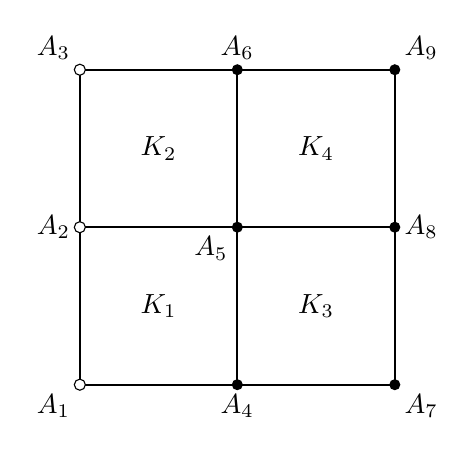
\begin{tikzpicture}[scale=2]

% 绘制矩形边界
\draw[thick] (-1,-1) rectangle (1,1);

% 网格步长
\def\step{1}

% 绘制网格线
\foreach \x in {-1,0,1} {
  \draw[thick] (\x,-1) -- (\x,1);
}
\foreach \y in {-1,0,1} {
  \draw[thick] (-1,\y) -- (1,\y);
}

% 节点位置列表(共9个)
\foreach \x in {-1,0,1} {
  \foreach \y in {-1,0,1} {
    % 判断是否画实心或空心点
    \pgfmathtruncatemacro{\isSolid}{ifthenelse(\x==-1,0,1)}
    % if x==-1, isSolid=0, else, isSolid=1
    \ifnum\isSolid=1
      \fill (\x,\y) circle (1pt); % 实心点
    \else
      \draw[fill=white] (\x,\y) circle (1pt); % 空心点
    \fi
  }
}
\node[below left] at (-1,-1) {${A}_1$};
\node[left] at (-1,0) {$A_2$};
\node[above left] at (-1,1) {$A_3$};
\node[below] at (0,-1) {$A_4$};
\node[below left] at (0,0) {$A_5$};
\node[above] at (0,1) {$A_6$};
\node[below right] at (1,-1) {$A_7$};
\node[right] at (1,0) {$A_8$};
\node[above right] at (1,1) {$A_9$};

\node at (-0.5,-0.5) {$K_1$};
\node at (-0.5,0.5) {$K_2$};
\node at (0.5,-0.5) {$K_3$};
\node at (0.5,0.5) {$K_4$};
\end{tikzpicture}
\caption{Mesh for $Q1-$FEM.}
\label{mesh1}
\end{figure}




\noindent For each $K_i$, we arrange its vertices in counterclockwise order starting from the bottom-left vertex. Thus it is clear that
\[
\begin{aligned}
& T_{K_1} (\hat{x},\hat{y}) = 
\begin{pmatrix}
\frac{1}{2} & 0 \\
0 & \frac{1}{2} \\
\end{pmatrix}
\begin{pmatrix}
\hat{x} \\
\hat{y} \\
\end{pmatrix}
+ 
\begin{pmatrix}
-\frac{1}{2} \\
-\frac{1}{2} 
\end{pmatrix}, \\
&
T_{K_2} (\hat{x},\hat{y}) = 
\begin{pmatrix}
\frac{1}{2} & 0 \\
0 & \frac{1}{2} \\
\end{pmatrix}
\begin{pmatrix}
\hat{x} \\
\hat{y} \\
\end{pmatrix}
+ 
\begin{pmatrix}
-\frac{1}{2} \\
\frac{1}{2} 
\end{pmatrix}, \\
&
T_{K_3} (\hat{x},\hat{y}) = 
\begin{pmatrix}
\frac{1}{2} & 0 \\
0 & \frac{1}{2} \\
\end{pmatrix}
\begin{pmatrix}
\hat{x} \\
\hat{y} \\
\end{pmatrix}
+ 
\begin{pmatrix}
\frac{1}{2} \\
-\frac{1}{2} 
\end{pmatrix}, \\
&
T_{K_4} (\hat{x},\hat{y}) = 
\begin{pmatrix}
\frac{1}{2} & 0 \\
0 & \frac{1}{2} \\
\end{pmatrix}
\begin{pmatrix}
\hat{x} \\
\hat{y} \\
\end{pmatrix}
+ 
\begin{pmatrix}
\frac{1}{2} \\
\frac{1}{2} 
\end{pmatrix}.
\end{aligned}
\]
The mapping from local basis functions $\{\hat{\phi}_i\}$ in \eqref{eq:basis-rec} to local part of $\psi_i$ gives
\[
\begin{aligned}
& \psi_1 |_{K_1} = (\hat{\phi}_1 \circ T_{K_1}^{-1} ) (x,y), \\
& \psi_2 |_{K_1} = (\hat{\phi}_4 \circ T_{K_1}^{-1} ) (x,y),\ \psi_2 |_{K_2} = (\hat{\phi}_1 \circ T_{K_2}^{-1} ) (x,y), \\
& \psi_3 |_{K_2} = (\hat{\phi}_4 \circ T_{K_2}^{-1} ) (x,y), \\
& \psi_4 |_{K_1}  = (\hat{\phi}_2 \circ T_{K_1}^{-1})(x,y),\ \psi_4 |_{K_3} = (\hat{\phi}_1 \circ T_{K_3}^{-1})(x,y),\\
& \psi_5 |_{K_1} = (\hat{\psi}_3 \circ T_{K_1}^{-1} )(x,y),\ \psi_5 |_{K_2} = (\hat{\phi}_2 \circ T_{K_2}^{-1})(x,y), \\
& \psi_5 |_{K_3} = (\hat{\phi}_4 \circ T_{K_3}^{-1})(x,y),\ \psi_5 |_{K_4} = (\hat{\phi}_1 \circ T_{K_1}^{-1})(x,y),\\
& \psi_6 |_{K_2} = (\hat{\phi}_3 \circ T_{K_2}^{-1})(x,y),\ \psi_6 |_{K_4} = (\hat{\phi}_4 \circ T_{K_4}^{-1}) (x,y), \\
& \psi_7 |_{K_3} = (\hat{\phi}_2 \circ T_{K_3}^{-1})(x,y), \\
& \psi_8 |_{K_3} = (\hat{\phi}_3 \circ T_{K_3}^{-1})(x,y),\ \psi_8 |_{K_4} = (\hat{\phi}_2 \circ T_{K_4}^{-1}) (x,y),\\
& \psi_{9} |_{K_4} = (\hat{\phi}_3 \circ T_{K_4}^{-1}) (x,y).
\end{aligned}
\]
Thus it is clear that the nodal basis are
\[
\psi_1 = 
\left \{
\begin{aligned}
& xy, & (x,y) \in K_1,\\
& 0, & else,
\end{aligned}
\right .
\
\psi_2 = 
\left \{
\begin{aligned}
& -x(1+y), & (x,y) \in K_1,\\
& -x(1-y), & (x,y) \in K_2, \\
& 0, & else,
\end{aligned}
\right .
\
\psi_3 = 
\left \{
\begin{aligned}
& -xy, & (x,y) \in K_2,\\
& 0, & else, 
\end{aligned}
\right .
\]
\[
\psi_4 = 
\left \{
\begin{aligned}
& -y(1+x), & (x,y) \in K_1, \\
& -y(1-x), & (x,y) \in K_3,\\
& 0, & else, 
\end{aligned}
\right .
\
\psi_5 = 
\left \{
\begin{aligned}
& (1+x)(1+y), & (x,y) \in K_1, \\
& (1+x)(1-y), & (x,y) \in K_2,\\
& (1-x)(1+y), & (x,y) \in K_3, \\
& (1-x)(1-y), & (x,y) \in K_4,\\
& 0, & else, 
\end{aligned}
\right .
\
\psi_6 = 
\left \{
\begin{aligned}
& y(1+x), & (x,y) \in K_2, \\
& y(1-x), & (x,y) \in K_4,\\
& 0, & else, 
\end{aligned}
\right .
\]
\[
\psi_7 = 
\left \{
\begin{aligned}
& -xy, & (x,y)\in K_3, \\
& 0, & else,
\end{aligned}
\right .
\
\psi_8 = 
\left \{
\begin{aligned}
& x(1+y), & (x,y)\in K_3, \\
& x(1-y), & (x,y)\in K_4,\\
& 0, & else,
\end{aligned}
\right .
\
\psi_9 = 
\left \{
\begin{aligned}
& xy, & (x,y)\in K_4, \\
& 0, & else.
\end{aligned}
\right .
\]
Thus we have $X_h^1 = \mathrm{span}\{\psi_1,\cdots,\psi_9\}$. Let $V_h = V \cap X_h^1 = \mathrm{span}\{\psi_4,\psi_5,\psi_6,\psi_7,\psi_8,\psi_9 \}$ and $u(x,y) = \sum_{j=4}^9 u_j \psi_j(x,y)$. Inserting $u$ into \eqref{eq:galerkin} gives the implementation of $Q1-$FEM
\[
\sum_{i=4}^9 a(\psi_j,\psi_i) u_j = \mathcal{F}(\psi_i),\quad i=4,5,6,7,8,9. 
\]

\vspace{1em}

\noindent $2.$ $P1-$FEM.
We relabel the subelements of Fig.~\subref{mesh-P1} as shown in Fig.~\ref{mesh2}, and define the finite element space 
\[
X_h^1 = \{v\in C(\bar{\Omega}): v|_{E_i} \in \mathbb{P}_1, \ i=1,\cdots,8\}.
\]
Next, we consider the basis functions for $X_h^1$. Let $\varphi_i$ for $i=1,\cdots,9$ denote the basis function associated with the node $B_i$.
The basis functions are constructed in a way: "reference basis" $\to$ "local basis" $\to$ "global basis". 

Let $T_{E_i}: \hat{E}\to E_i$ denote the affine mapping from the reference element  $\hat{E}$ in Fig.~\ref{tri-ref2gen} to physical element $E_i$ in Fig.~\ref{mesh2} for $i=1,\cdots,8$. The exact expression of $T_{E_i}$ is given in \eqref{eq:affine-tri}. 

\begin{figure}[H]
\centering
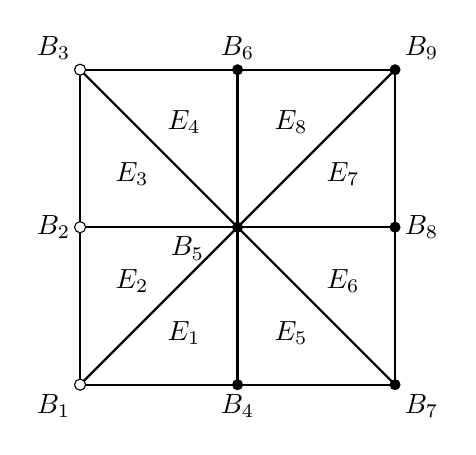
\begin{tikzpicture}[scale=2]

% 绘制矩形边界
\draw[thick] (-1,-1) rectangle (1,1);

% 网格步长
\def\step{1}

% 绘制网格线
\foreach \x in {-1,0,1} {
  \draw[thick] (\x,-1) -- (\x,1);
}
\foreach \y in {-1,0,1} {
  \draw[thick] (-1,\y) -- (1,\y);
}
\draw[thick] (-1,-1) -- (1,1);
\draw[thick] (-1,1) -- (1,-1);


% 节点位置列表(共9个)
\foreach \x in {-1,0,1} {
  \foreach \y in {-1,0,1} {
    % 判断是否画实心或空心点
    \pgfmathtruncatemacro{\isSolid}{ifthenelse(\x==-1,0,1)}
    % if x==-1, isSolid=0, else, isSolid=1
    \ifnum\isSolid=1
      \fill (\x,\y) circle (1pt); % 实心点
    \else
      \draw[fill=white] (\x,\y) circle (1pt); % 空心点
    \fi
  }
}
\node[below left] at (-1,-1) {${B}_1$};
\node[left] at (-1,0) {$B_2$};
\node[above left] at (-1,1) {$B_3$};
\node[below] at (0,-1) {$B_4$};
\node[below left] at (-0.15,0) {$B_5$};
\node[above] at (0,1) {$B_6$};
\node[below right] at (1,-1) {$B_7$};
\node[right] at (1,0) {$B_8$};
\node[above right] at (1,1) {$B_9$};

\node at (-0.34,-0.67) {$E_1$};
\node at (-0.67,-0.34) {$E_2$};
\node at (-0.67,0.34) {$E_3$};
\node at (-0.34,0.67) {$E_4$};
\node at (0.34,-0.67) {$E_5$};
\node at (0.67,-0.34) {$E_6$};
\node at (0.67, 0.34) {$E_7$};
\node at (0.34,0.67) {$E_8$};
\end{tikzpicture}
\caption{Mesh for $P1-$FEM.}
\label{mesh2}
\end{figure}


\noindent For each element $E_i$, we arrange its vertices in counterclockwise order, starting from the right-angled vertex. For example, the vertices of  the element $E_1$ are $\{B_1, B_4, B_5\}$, then we map from $\hat{E}: \Delta \hat{B}_1\hat{B}_2\hat{B}_3$ to $E_1: \Delta B_4 B_5 B_1$ shown as

\begin{figure}[H]
\centering
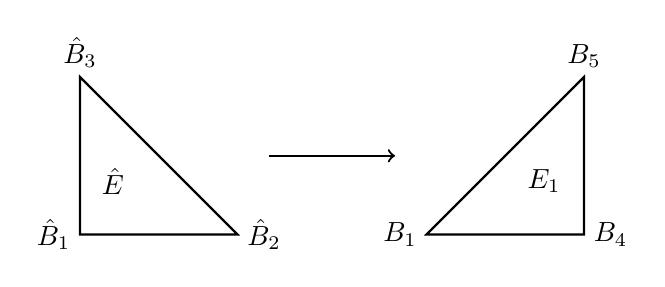
\begin{tikzpicture}[scale=2]

% 参考矩形(单位矩形)
\coordinate (hatB1) at (0,0);
\coordinate (hatB2) at (1,0);
\coordinate (hatB3) at (0,1);
\coordinate (hatcen) at (0.34,0.34);

% 一般矩形(变形后的)
\coordinate (B1) at (2.2, 0);
\coordinate (B2) at (3.2,0);
\coordinate (B3) at (3.2,1);
\coordinate (cen) at (2.78,0.34);

% 绘制参考矩形
\draw[thick, black] (hatB1) -- (hatB2) -- (hatB3) -- cycle;
\node[left] at (hatB1) {$\hat{B}_1$};
\node[right] at (hatB2) {$\hat{B}_2$};
\node[above] at (hatB3) {$\hat{B}_3$};
\node[left] at (hatcen) {$\hat{E}$};

% 绘制一般矩形
\draw[thick, black] (B1) -- (B2) -- (B3)  -- cycle;
\node[left] at (B1) {$B_1$};
\node[right] at (B2) {$B_4$};
\node[above] at (B3) {$B_5$};
\node[right] at (cen) {${E}_1$};

% 映射箭头
\draw[->, thick] (1.2,0.5) -- (2,0.5);



\end{tikzpicture}
\end{figure}

\noindent Thus it is clear that 
\[
\begin{aligned}
& T_{E_1}(\hat{x},\hat{y}) = 
\begin{pmatrix}
0 & -1 \\
1 & 0 
\end{pmatrix}
\begin{pmatrix}
\hat{x} \\
\hat{y}
\end{pmatrix}
+
\begin{pmatrix}
0 \\
-1
\end{pmatrix}, 
\quad
T_{E_2}(\hat{x},\hat{y}) = 
\begin{pmatrix}
0 & 1 \\
-1 & 0 
\end{pmatrix}
\begin{pmatrix}
\hat{x} \\
\hat{y}
\end{pmatrix}
+
\begin{pmatrix}
-1 \\
0
\end{pmatrix}, \\
&
T_{E_3}(\hat{x},\hat{y}) = 
\begin{pmatrix}
1 & 0 \\
0 & 1 
\end{pmatrix}
\begin{pmatrix}
\hat{x} \\
\hat{y}
\end{pmatrix}
+
\begin{pmatrix}
-1 \\
0
\end{pmatrix}, 
\quad \ \
T_{E_4}(\hat{x},\hat{y}) = 
\begin{pmatrix}
-1 & 0 \\
0 & -1 
\end{pmatrix}
\begin{pmatrix}
\hat{x} \\
\hat{y}
\end{pmatrix}
+
\begin{pmatrix}
0 \\
1
\end{pmatrix}, \\
& 
T_{E_5}(\hat{x},\hat{y}) = 
\begin{pmatrix}
1 & 0 \\
0 & 1 
\end{pmatrix}
\begin{pmatrix}
\hat{x} \\
\hat{y}
\end{pmatrix}
+
\begin{pmatrix}
0 \\
-1
\end{pmatrix}, 
\quad \ \ 
T_{E_6}(\hat{x},\hat{y}) = 
\begin{pmatrix}
-1 & 0 \\
0 & -1 
\end{pmatrix}
\begin{pmatrix}
\hat{x} \\
\hat{y}
\end{pmatrix}
+
\begin{pmatrix}
1 \\
0
\end{pmatrix}, \\
&
T_{E_7}(\hat{x},\hat{y}) = 
\begin{pmatrix}
0 & -1 \\
1 & 0 
\end{pmatrix}
\begin{pmatrix}
\hat{x} \\
\hat{y}
\end{pmatrix}
+
\begin{pmatrix}
1 \\
0
\end{pmatrix}, 
\quad \ \
T_{E_8}(\hat{x},\hat{y}) = 
\begin{pmatrix}
0 & 1 \\
-1 & 0 
\end{pmatrix}
\begin{pmatrix}
\hat{x} \\
\hat{y}
\end{pmatrix}
+
\begin{pmatrix}
0 \\
1
\end{pmatrix}.
\end{aligned}
\]
The mapping from local basis functions $\{\hat{\eta}_i\}$ in \eqref{eq:basis-tri} to local part of $\varphi_i$ gives
\[
\begin{aligned}
& \varphi_1 |_{E_1} = \left( \hat{\eta}_3 \circ T_{E_1}^{-1} \right )(x,y),\
\varphi_1 |_{E_2} = \left( \hat{\eta}_2 \circ T_{E_2}^{-1} \right )(x,y), \\
& \varphi_2 |_{E_2} = \left( \hat{\eta}_1 \circ T_{E_2}^{-1} \right )(x,y), \
\varphi_2 |_{E_3} = \left( \hat{\eta}_1 \circ T_{E_3}^{-1} \right )(x,y), \\
& \varphi_3 |_{E_3} = \left( \hat{\eta}_3 \circ T_{E_3}^{-1} \right )(x,y),\
\varphi_3 |_{E_4} = \left( \hat{\eta}_2 \circ T_{E_4}^{-1} \right )(x,y), \\
& \varphi_4 |_{E_1} = \left( \hat{\eta}_1 \circ T_{E_1}^{-1} \right )(x,y), \
\varphi_4 |_{E_5} = \left( \hat{\eta}_1 \circ T_{E_5}^{-1} \right )(x,y), \\
& \varphi_5 |_{E_1} = \left( \hat{\eta}_2 \circ T_{E_1}^{-1} \right )(x,y), \
\varphi_5 |_{E_2} = \left( \hat{\eta}_3 \circ T_{E_2}^{-1} \right )(x,y), \\
& \varphi_5 |_{E_3} = \left( \hat{\eta}_2 \circ T_{E_3}^{-1} \right )(x,y),\
\varphi_5 |_{E_4} = \left( \hat{\eta}_3 \circ T_{E_4}^{-1} \right )(x,y), \\
& \varphi_5 |_{E_5} = \left( \hat{\eta}_3 \circ T_{E_5}^{-1} \right )(x,y), \
\varphi_5 |_{E_6} = \left( \hat{\eta}_2 \circ T_{E_6}^{-1} \right )(x,y), \\
& \varphi_5 |_{E_7} = \left( \hat{\eta}_3 \circ T_{E_7}^{-1} \right )(x,y),\
\varphi_5 |_{E_8} = \left( \hat{\eta}_2 \circ T_{E_8}^{-1} \right )(x,y), \\
& \varphi_6 |_{E_4} = \left( \hat{\eta}_1 \circ T_{E_4}^{-1} \right )(x,y), \
\varphi_6 |_{E_8} = \left( \hat{\eta}_1 \circ T_{E_8}^{-1} \right )(x,y), \\
& \varphi_7 |_{E_5} = \left( \hat{\eta}_2 \circ T_{E_5}^{-1} \right )(x,y), \
\varphi_7 |_{E_6} = \left( \hat{\eta}_3 \circ T_{E_6}^{-1} \right )(x,y), \\
& \varphi_8 |_{E_6} = \left( \hat{\eta}_1 \circ T_{E_6}^{-1} \right )(x,y),\
\varphi_8 |_{E_7} = \left( \hat{\eta}_1 \circ T_{E_7}^{-1} \right )(x,y), \\
& \varphi_9 |_{E_7} = \left( \hat{\eta}_2 \circ T_{E_7}^{-1} \right )(x,y),\
\varphi_9 |_{E_8} = \left( \hat{\eta}_3 \circ T_{E_8}^{-1} \right )(x,y).
\end{aligned}
\]
Thus it is clear that the nodal basis are
\[
\begin{aligned}
& \varphi_1(x,y) = 
\left\{
\begin{aligned}
& -x, & (x,y)\in E_1, \\
& -y, & (x,y) \in E_2,\\
& 0, & else,
\end{aligned}
\right .
\
\varphi_2(x,y) = 
\left\{
\begin{aligned}
& y-x, & (x,y)\in E_2, \\
& -x-y, & (x,y) \in E_3,\\
& 0, & else,
\end{aligned}
\right .
\\
& 
\varphi_3(x,y) = 
\left\{
\begin{aligned}
& y, & (x,y)\in E_3, \\
& -x, & (x,y) \in E_4,\\
& 0, & else,
\end{aligned}
\right .
\
\varphi_4(x,y) = 
\left\{
\begin{aligned}
& x-y, & (x,y)\in E_1, \\
& -x-y, & (x,y) \in E_5,\\
& 0, & else,
\end{aligned}
\right .
\\
&
\varphi_6(x,y) = 
\left\{
\begin{aligned}
& x+y, & (x,y)\in E_4, \\
& y-x, & (x,y) \in E_8,\\
& 0, & else,
\end{aligned}
\right .
\
\varphi_7(x,y) = 
\left\{
\begin{aligned}
& x, & (x,y)\in E_5, \\
& -y, & (x,y) \in E_6,\\
& 0, & else,
\end{aligned}
\right .
\\
&
\varphi_8(x,y) = 
\left\{
\begin{aligned}
& x+y, & (x,y)\in E_6, \\
& x-y, & (x,y) \in E_7,\\
& 0, & else,
\end{aligned}
\right .
\
\varphi_9(x,y) = 
\left\{
\begin{aligned}
& y, & (x,y)\in E_7, \\
& x, & (x,y) \in E_8,\\
& 0, & else,
\end{aligned}
\right .
\\
& 
\varphi_5(x,y) = 
\left\{
\begin{aligned}
& 1+y, & (x,y)\in E_1, \\
& 1+x, & (x,y) \in E_2,\\
& 1+x, & (x,y)\in E_3, \\
& 1-y, & (x,y) \in E_4,\\
& 1+y, & (x,y)\in E_5, \\
& 1-x, & (x,y) \in E_6,\\
& 1-x, & (x,y)\in E_7, \\
& 1-y, & (x,y) \in E_8.\\
\end{aligned}
\right .
\end{aligned}
\]
Thus we have $X_h^1 = \mathrm{span}\{\varphi_1,\cdots,\psi_9\}$. Let $V_h = V \cap X_h^1 = \mathrm{span}\{\varphi_4,\varphi_5,\varphi_6,\varphi_7,\varphi_8,\varphi_9 \}$ and $u(x,y) = \sum_{j=4}^9 u_j \varphi_j(x,y)$. Inserting $u$ into \eqref{eq:galerkin} gives the implementation of $P1-$FEM
\[
\sum_{i=4}^9 a(\varphi_j,\varphi_i) u_j = \mathcal{F}(\varphi_i),\quad i=4,5,6,7,8,9. 
\]

\end{proof}





\newpage
\section*{Appendix}

\appendix

\numberwithin{equation}{section}
\numberwithin{figure}{section}
\section{Affine mapping between rectangles}
Let the reference rectangle $\hat{K}$ with its vertices $\hat{A}_1=(-1,-1)$, $\hat{A}_2=(1,-1)$, $\hat{A}_3 = (1,1)$ and $\hat{A}_4 = (-1,1)$. For any physical rectangle $K$ with vertices $A_1$, $A_2$, $A_3$ and $A_4$, the affine mapping from $\hat{K}$ to $K$ is shown as follows

\begin{figure}[H]
\centering
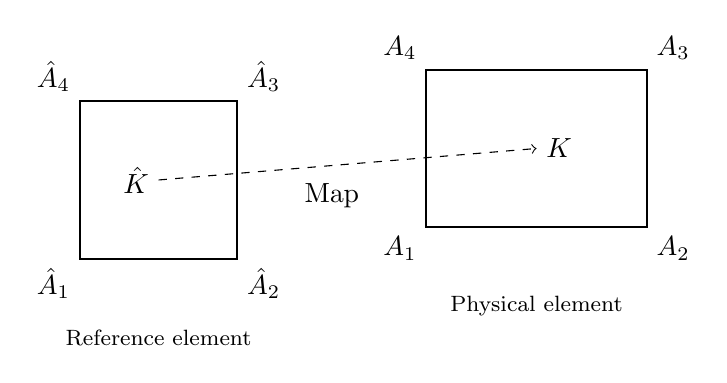
\begin{tikzpicture}[scale=2]

% 参考矩形(单位矩形)
\coordinate (hatA1) at (0,0);
\coordinate (hatA2) at (1,0);
\coordinate (hatA3) at (1,1);
\coordinate (hatA4) at (0,1);
\coordinate (hatcen) at (0.5,0.5);

% 一般矩形(变形后的)
\coordinate (A1) at (2.2,0.2);
\coordinate (A2) at (3.6,0.2);
\coordinate (A3) at (3.6,1.2);
\coordinate (A4) at (2.2,1.2);
\coordinate (cen) at (2.9,0.7);

% 绘制参考矩形
\draw[thick, black] (hatA1) -- (hatA2) -- (hatA3) -- (hatA4) -- cycle;
\node[below left] at (hatA1) {$\hat{A}_1$};
\node[below right] at (hatA2) {$\hat{A}_2$};
\node[above right] at (hatA3) {$\hat{A}_3$};
\node[above left] at (hatA4) {$\hat{A}_4$};
\node[left] at (hatcen) {$\hat{K}$};

% 绘制一般矩形
\draw[thick, black] (A1) -- (A2) -- (A3) -- (A4) -- cycle;
\node[below left] at (A1) {$A_1$};
\node[below right] at (A2) {$A_2$};
\node[above right] at (A3) {$A_3$};
\node[above left] at (A4) {$A_4$};
\node[right] at (cen) {${K}$};

% 映射箭头
\draw[->, dashed] (hatcen) -- (cen);


% 映射说明
\node at (0.5, -0.5) {\footnotesize Reference element};
\node at (2.9, -0.3) {\footnotesize Physical element};
\node at (1.6, 0.4) {Map};

\end{tikzpicture}
\caption{Affine mapping from the reference element $\hat{K}$ to a physical element $K$.}
\label{rec-ref2gen}
\end{figure}

$Q1-$basis on element $\hat{K}=\Box \hat{A}_1\hat{A}_2\hat{A}_3\hat{A}_4$ is denoted as $\{\hat{\phi}_i\}_{i=1}^4$, each of which corresponds to the node $\hat{A}_i$, satisfying $\hat{\phi}_i(\hat{A}_j) = \delta_{ij}$. It is clear that
\begin{equation}
\begin{aligned}
& \hat{\phi}_1(\hat{x},\hat{y}) = \frac{1-\hat{x}-\hat{y}+\hat{x}\hat{y}}{4}, \\
& \hat{\phi}_2(\hat{x},\hat{y}) = \frac{1+\hat{x}-\hat{y}-\hat{x}\hat{y}}{4}, \\
& \hat{\phi}_3(\hat{x},\hat{y}) = \frac{1+\hat{x}+\hat{y}+\hat{x}\hat{y}}{4}, \\
& \hat{\phi}_4(\hat{x},\hat{y}) = \frac{1-\hat{x}+\hat{y}-\hat{x}\hat{y}}{4}.
\end{aligned}
\label{eq:basis-rec}
\end{equation}
Assume that $K=\Box A_1A_2A_3A_4$ is an arbitrary rectangle with the coordinates 
\[
A_i = 
\begin{pmatrix}
x_i \\
y_i
\end{pmatrix},
\
i=1,2,3,4.
\]
Then the affine mapping from $\hat{K}$ to $K$ is 
\begin{equation}
\begin{pmatrix}
x\\
y
\end{pmatrix}
=
T_K(\hat{x},\hat{y}) =
\begin{pmatrix}
\frac{1}{2}h_1 & 0 \\
0 & \frac{1}{2} h_2\\
\end{pmatrix}
\begin{pmatrix}
\hat{x} \\
\hat{y}
\end{pmatrix}
+
\begin{pmatrix}
x_1+\frac{1}{2} h_1 \\
y_1 + \frac{1}{2} h_2
\end{pmatrix},
\label{eq:affine-rec}
\end{equation}
where $h_1 = x_2-x_1,\ h_2 = y_4-y_1$.


\newpage
\section{Affine mapping between triangles}

Let the reference triangle $\hat{E}$ with its vertices $\hat{B}_1 = (0,0)$, $\hat{B}_2 = (1,0)$, and $\hat{B}_3 = (0,1)$. For any physical triangle $E$ with vertices $B_1$, $B_2$, and $B_3$, the affine mapping from $\hat{E}$ to $E$ is shown as follows

\begin{figure}[H]
\centering
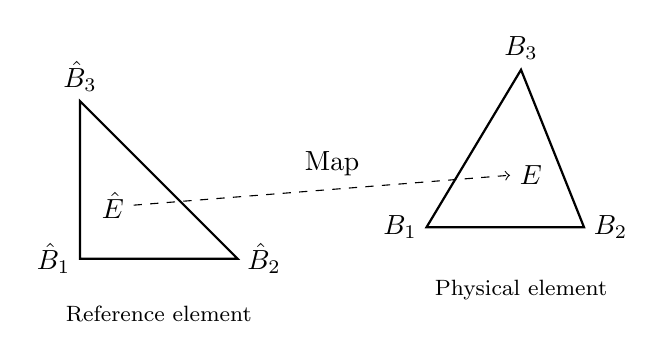
\begin{tikzpicture}[scale=2]

% 参考矩形(单位矩形)
\coordinate (hatB1) at (0,0);
\coordinate (hatB2) at (1,0);
\coordinate (hatB3) at (0,1);
\coordinate (hatcen) at (0.34,0.34);

% 一般矩形(变形后的)
\coordinate (B1) at (2.2,0.2);
\coordinate (B2) at (3.2,0.2);
\coordinate (B3) at (2.8,1.2);
\coordinate (cen) at (2.73,0.53);

% 绘制参考矩形
\draw[thick, black] (hatB1) -- (hatB2) -- (hatB3) -- cycle;
\node[left] at (hatB1) {$\hat{B}_1$};
\node[right] at (hatB2) {$\hat{B}_2$};
\node[above] at (hatB3) {$\hat{B}_3$};
\node[left] at (hatcen) {$\hat{E}$};

% 绘制一般矩形
\draw[thick, black] (B1) -- (B2) -- (B3)  -- cycle;
\node[left] at (B1) {$B_1$};
\node[right] at (B2) {$B_2$};
\node[above] at (B3) {$B_3$};
\node[right] at (cen) {${E}$};

% 映射箭头
\draw[->, dashed] (hatcen) -- (cen);


% 映射说明
\node at (0.5, -0.35) {\footnotesize Reference element};
\node at (2.8, -0.2) {\footnotesize Physical element};
\node at (1.6, 0.6) {Map};

\end{tikzpicture}
\caption{Affine mapping from the reference element $\hat{E}$ to a physical element $E$.}
\label{tri-ref2gen}
\end{figure}

$P1-$basis on element $\hat{E}=\Delta \hat{B}_1\hat{B}_2\hat{B}_3$ is denoted as $\{\hat{\eta}_i\}_{i=1}^3$, each of which corresponds to the node $\hat{B}_i$, satisfying $\hat{\eta}_i(\hat{B}_j) = \delta_{ij}$. It is clear that

\begin{equation}
\begin{aligned}
& \hat{\eta}_1(\hat{x},\hat{y}) =  -\hat{x}-\hat{y}+1, \\
& \hat{\eta}_2 (\hat{x},\hat{y}) = \hat{x}, \\
& \hat{\eta}_3 (\hat{x},\hat{y}) = \hat{y}.
\end{aligned}
\label{eq:basis-tri}
\end{equation}
Assume that for an arbitrary triangle $E = \Delta B_1 B_2 B_3$ with the coordinates
\[
B_i = 
\begin{pmatrix}
x_i \\
y_i
\end{pmatrix},
\quad  i = 1,2,3.
\]
The affine mapping from $\hat{K}$ to $K$ is 
\begin{equation}
\begin{pmatrix}
x \\
y
\end{pmatrix}
=
T_K(\hat{x}, \hat{y}) 
=
\begin{pmatrix}
x_2- x_1 & x_3 - x_1 \\
y_2 - y_1 & y_3 - y_1
\end{pmatrix}
\begin{pmatrix}
\hat{x} \\
\hat{y}
\end{pmatrix}
+
\begin{pmatrix}
{x}_1 \\
{y}_1
\end{pmatrix}.
\label{eq:affine-tri}
\end{equation}

\end{document}

